\documentclass[]{book}
\usepackage{lmodern}
\usepackage{amssymb,amsmath}
\usepackage{ifxetex,ifluatex}
\usepackage{fixltx2e} % provides \textsubscript
\ifnum 0\ifxetex 1\fi\ifluatex 1\fi=0 % if pdftex
  \usepackage[T1]{fontenc}
  \usepackage[utf8]{inputenc}
\else % if luatex or xelatex
  \ifxetex
    \usepackage{mathspec}
  \else
    \usepackage{fontspec}
  \fi
  \defaultfontfeatures{Ligatures=TeX,Scale=MatchLowercase}
\fi
% use upquote if available, for straight quotes in verbatim environments
\IfFileExists{upquote.sty}{\usepackage{upquote}}{}
% use microtype if available
\IfFileExists{microtype.sty}{%
\usepackage{microtype}
\UseMicrotypeSet[protrusion]{basicmath} % disable protrusion for tt fonts
}{}
\usepackage[margin=1in]{geometry}
\usepackage{hyperref}
\hypersetup{unicode=true,
            pdftitle={Data Science for Biological, Medical and Health Research: Notes for 432},
            pdfauthor={Thomas E. Love, Ph.D.},
            pdfborder={0 0 0},
            breaklinks=true}
\urlstyle{same}  % don't use monospace font for urls
\usepackage{natbib}
\bibliographystyle{apalike}
\usepackage{color}
\usepackage{fancyvrb}
\newcommand{\VerbBar}{|}
\newcommand{\VERB}{\Verb[commandchars=\\\{\}]}
\DefineVerbatimEnvironment{Highlighting}{Verbatim}{commandchars=\\\{\}}
% Add ',fontsize=\small' for more characters per line
\usepackage{framed}
\definecolor{shadecolor}{RGB}{248,248,248}
\newenvironment{Shaded}{\begin{snugshade}}{\end{snugshade}}
\newcommand{\KeywordTok}[1]{\textcolor[rgb]{0.13,0.29,0.53}{\textbf{#1}}}
\newcommand{\DataTypeTok}[1]{\textcolor[rgb]{0.13,0.29,0.53}{#1}}
\newcommand{\DecValTok}[1]{\textcolor[rgb]{0.00,0.00,0.81}{#1}}
\newcommand{\BaseNTok}[1]{\textcolor[rgb]{0.00,0.00,0.81}{#1}}
\newcommand{\FloatTok}[1]{\textcolor[rgb]{0.00,0.00,0.81}{#1}}
\newcommand{\ConstantTok}[1]{\textcolor[rgb]{0.00,0.00,0.00}{#1}}
\newcommand{\CharTok}[1]{\textcolor[rgb]{0.31,0.60,0.02}{#1}}
\newcommand{\SpecialCharTok}[1]{\textcolor[rgb]{0.00,0.00,0.00}{#1}}
\newcommand{\StringTok}[1]{\textcolor[rgb]{0.31,0.60,0.02}{#1}}
\newcommand{\VerbatimStringTok}[1]{\textcolor[rgb]{0.31,0.60,0.02}{#1}}
\newcommand{\SpecialStringTok}[1]{\textcolor[rgb]{0.31,0.60,0.02}{#1}}
\newcommand{\ImportTok}[1]{#1}
\newcommand{\CommentTok}[1]{\textcolor[rgb]{0.56,0.35,0.01}{\textit{#1}}}
\newcommand{\DocumentationTok}[1]{\textcolor[rgb]{0.56,0.35,0.01}{\textbf{\textit{#1}}}}
\newcommand{\AnnotationTok}[1]{\textcolor[rgb]{0.56,0.35,0.01}{\textbf{\textit{#1}}}}
\newcommand{\CommentVarTok}[1]{\textcolor[rgb]{0.56,0.35,0.01}{\textbf{\textit{#1}}}}
\newcommand{\OtherTok}[1]{\textcolor[rgb]{0.56,0.35,0.01}{#1}}
\newcommand{\FunctionTok}[1]{\textcolor[rgb]{0.00,0.00,0.00}{#1}}
\newcommand{\VariableTok}[1]{\textcolor[rgb]{0.00,0.00,0.00}{#1}}
\newcommand{\ControlFlowTok}[1]{\textcolor[rgb]{0.13,0.29,0.53}{\textbf{#1}}}
\newcommand{\OperatorTok}[1]{\textcolor[rgb]{0.81,0.36,0.00}{\textbf{#1}}}
\newcommand{\BuiltInTok}[1]{#1}
\newcommand{\ExtensionTok}[1]{#1}
\newcommand{\PreprocessorTok}[1]{\textcolor[rgb]{0.56,0.35,0.01}{\textit{#1}}}
\newcommand{\AttributeTok}[1]{\textcolor[rgb]{0.77,0.63,0.00}{#1}}
\newcommand{\RegionMarkerTok}[1]{#1}
\newcommand{\InformationTok}[1]{\textcolor[rgb]{0.56,0.35,0.01}{\textbf{\textit{#1}}}}
\newcommand{\WarningTok}[1]{\textcolor[rgb]{0.56,0.35,0.01}{\textbf{\textit{#1}}}}
\newcommand{\AlertTok}[1]{\textcolor[rgb]{0.94,0.16,0.16}{#1}}
\newcommand{\ErrorTok}[1]{\textcolor[rgb]{0.64,0.00,0.00}{\textbf{#1}}}
\newcommand{\NormalTok}[1]{#1}
\usepackage{longtable,booktabs}
\usepackage{graphicx,grffile}
\makeatletter
\def\maxwidth{\ifdim\Gin@nat@width>\linewidth\linewidth\else\Gin@nat@width\fi}
\def\maxheight{\ifdim\Gin@nat@height>\textheight\textheight\else\Gin@nat@height\fi}
\makeatother
% Scale images if necessary, so that they will not overflow the page
% margins by default, and it is still possible to overwrite the defaults
% using explicit options in \includegraphics[width, height, ...]{}
\setkeys{Gin}{width=\maxwidth,height=\maxheight,keepaspectratio}
\IfFileExists{parskip.sty}{%
\usepackage{parskip}
}{% else
\setlength{\parindent}{0pt}
\setlength{\parskip}{6pt plus 2pt minus 1pt}
}
\setlength{\emergencystretch}{3em}  % prevent overfull lines
\providecommand{\tightlist}{%
  \setlength{\itemsep}{0pt}\setlength{\parskip}{0pt}}
\setcounter{secnumdepth}{5}
% Redefines (sub)paragraphs to behave more like sections
\ifx\paragraph\undefined\else
\let\oldparagraph\paragraph
\renewcommand{\paragraph}[1]{\oldparagraph{#1}\mbox{}}
\fi
\ifx\subparagraph\undefined\else
\let\oldsubparagraph\subparagraph
\renewcommand{\subparagraph}[1]{\oldsubparagraph{#1}\mbox{}}
\fi

%%% Use protect on footnotes to avoid problems with footnotes in titles
\let\rmarkdownfootnote\footnote%
\def\footnote{\protect\rmarkdownfootnote}

%%% Change title format to be more compact
\usepackage{titling}

% Create subtitle command for use in maketitle
\newcommand{\subtitle}[1]{
  \posttitle{
    \begin{center}\large#1\end{center}
    }
}

\setlength{\droptitle}{-2em}
  \title{Data Science for Biological, Medical and Health Research: Notes for 432}
  \pretitle{\vspace{\droptitle}\centering\huge}
  \posttitle{\par}
  \author{Thomas E. Love, Ph.D.}
  \preauthor{\centering\large\emph}
  \postauthor{\par}
  \predate{\centering\large\emph}
  \postdate{\par}
  \date{Version: 2018-01-15}

\usepackage{booktabs}
\usepackage{amsthm}
\makeatletter
\def\thm@space@setup{%
  \thm@preskip=8pt plus 2pt minus 4pt
  \thm@postskip=\thm@preskip
}
\makeatother

\usepackage{amsthm}
\newtheorem{theorem}{Theorem}[chapter]
\newtheorem{lemma}{Lemma}[chapter]
\theoremstyle{definition}
\newtheorem{definition}{Definition}[chapter]
\newtheorem{corollary}{Corollary}[chapter]
\newtheorem{proposition}{Proposition}[chapter]
\theoremstyle{definition}
\newtheorem{example}{Example}[chapter]
\theoremstyle{definition}
\newtheorem{exercise}{Exercise}[chapter]
\theoremstyle{remark}
\newtheorem*{remark}{Remark}
\newtheorem*{solution}{Solution}
\begin{document}
\maketitle

{
\setcounter{tocdepth}{1}
\tableofcontents
}
\chapter*{Introduction}\label{introduction}
\addcontentsline{toc}{chapter}{Introduction}

These Notes provide a series of examples using R to work through issues
that are likely to come up in PQHS/CRSP/MPHP 432.

While these Notes share some of the features of a textbook, they are
neither comprehensive nor completely original. The main purpose is to
give 432 students a set of common materials on which to draw during the
course. In class, we will sometimes:

\begin{itemize}
\tightlist
\item
  reiterate points made in this document,
\item
  amplify what is here,
\item
  simplify the presentation of things done here,
\item
  use new examples to show some of the same techniques,
\item
  refer to issues not mentioned in this document,
\end{itemize}

but what we don't do is follow these notes very precisely. We assume
instead that you will read the materials and try to learn from them,
just as you will attend classes and try to learn from them. We welcome
feedback of all kinds on this document or anything else. Just email us
at \texttt{431-help\ at\ case\ dot\ edu}, or submit a pull request.

What you will mostly find are brief explanations of a key idea or
summary, accompanied (most of the time) by R code and a demonstration of
the results of applying that code.

Everything you see here is available to you as HTML or PDF. You will
also have access to the R Markdown files, which contain the code which
generates everything in the document, including all of the R results. We
will demonstrate the use of R Markdown (this document is generated with
the additional help of an R package called bookdown) and R Studio (the
``program'' which we use to interface with the R language) in class.

To download the data and R code related to these notes, visit the Data
and Code section of \href{https://github.com/THOMASELOVE/432-2018}{the
432 course website}.

\chapter*{R Packages used in these
notes}\label{r-packages-used-in-these-notes}
\addcontentsline{toc}{chapter}{R Packages used in these notes}

Here, we'll load in the packages used in these notes.

\begin{Shaded}
\begin{Highlighting}[]
\KeywordTok{library}\NormalTok{(tableone); }\KeywordTok{library}\NormalTok{(tidyverse)}
\end{Highlighting}
\end{Shaded}

\chapter*{Data used in these notes}\label{data-used-in-these-notes}
\addcontentsline{toc}{chapter}{Data used in these notes}

Here, we'll load in the data sets used in these notes.

\begin{Shaded}
\begin{Highlighting}[]
\NormalTok{fakestroke <-}\StringTok{ }\KeywordTok{read.csv}\NormalTok{(}\StringTok{"data/fakestroke.csv"}\NormalTok{) }\OperatorTok\StringTok{ }\NormalTok{tbl_df}
\end{Highlighting}
\end{Shaded}

\chapter{Building Table 1}\label{building-table-1}

Many scientific articles involve direct comparison of results from
various exposures, perhaps treatments. In 431, we studied numerous
methods, including various sorts of hypothesis tests, confidence
intervals, and descriptive summaries, which can help us to understand
and compare outcomes in such a setting. One common approach is to
present what's often called Table 1. Table 1 provides a summary of the
characteristics of a sample, or of groups of samples, which is most
commonly used to help understand the nature of the data being compared.

\section{Two examples from the New England Journal of
Medicine}\label{two-examples-from-the-new-england-journal-of-medicine}

\subsection{A simple Table 1}\label{a-simple-table-1}

Table 1 is especially common in the context of clinical research.
Consider the excerpt below, from a January 2015 article in the \emph{New
England Journal of Medicine} \citep{Tolaney2015}.

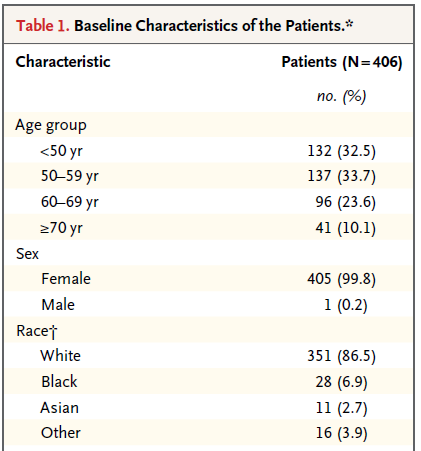
\includegraphics[width=0.5\linewidth]{images/Tolaney-snip1}

This (partial) table reports baseline characteristics on age group, sex
and race, describing 406 patients with HER2-positive\footnote{HER2 =
  human epidermal growth factor receptor type 2. Over-expression of this
  occurs in 15-20\% of invasive breast cancers, and has been associated
  with poor outcomes.} invasive breast cancer that began the protocol
therapy. Age, sex and race (along with severity of illness) are the most
commonly identified characteristics in a Table 1.

In addition to the measures shown in this excerpt, the full Table also
includes detailed information on the primary tumor for each patient,
including its size, nodal status and histologic grade. Footnotes tell us
that the percentages shown are subject to rounding, and may not total
100, and that the race information was self-reported.

\subsection{Table 1 showing a group
comparison}\label{table-1-showing-a-group-comparison}

A more typical Table 1 involves a group comparison, for example in this
excerpt from \citet{Roy2008}. This Table 1 describes a multi-center
randomized clinical trial comparing two different approaches to caring
for patients with heart failure and atrial fibrillation\footnote{The
  complete Table 1 appears on pages 2668-2669 of \citet{Roy2008}, but I
  have only reproduced the first page and the footnote in this excerpt.}.

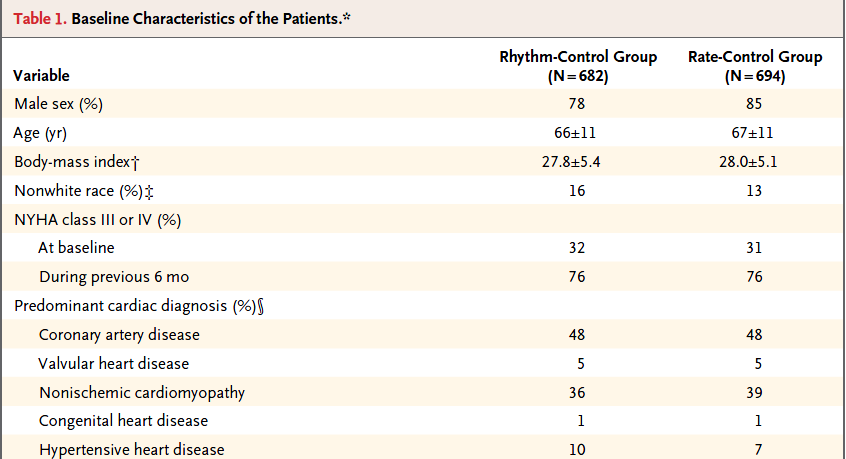
\includegraphics[width=0.9\linewidth]{images/Roy-snip1}

The article provides percentages, means and standard deviations across
groups, but note that it does not provide p values for the comparison of
baseline characteristics. This is a common feature of NEJM reports on
randomized clinical trials, where we anticipate that the two groups will
be well matched at baseline. Note that the patients in this study were
\emph{randomly} assigned to either the rhythm-control group or to the
rate-control group, using blocked randomizations stratified by study
center.

\section{Simulating Data from a Clinical
Trial}\label{simulating-data-from-a-clinical-trial}

Consider the following simulated data, available on the Data and Code
page of \href{https://github.com/THOMASELOVE/432-2018}{our course
website} in the \texttt{fakestroke.csv} file, which I built to let us
mirror the Table 1 for a real randomized clinical trial, called MR CLEAN
\citep{Berkheimer2015}.

The MR CLEAN trial report describes 500 patients with acute ischemic
stroke at 16 medical centers in the Netherlands, where 233 were randomly
assigned to the intervention (intraarterial treatment plus usual care)
and 267 to control (usual care alone.)

\subsection{\texorpdfstring{The \texttt{fakestroke}
data}{The fakestroke data}}\label{the-fakestroke-data}

Here's a quick look at the simulated data in \texttt{fakestroke}.

\begin{Shaded}
\begin{Highlighting}[]
\NormalTok{fakestroke}
\end{Highlighting}
\end{Shaded}

\begin{verbatim}
# A tibble: 500 x 18
   studyid trt        age sex   nihss location hx.isch  afib    dm mrankin
   <fct>   <fct>    <dbl> <fct> <int> <fct>    <fct>   <int> <int> <fct>  
 1 z001    Control   53.0 Male     21 Right    No          0     0 2      
 2 z002    Interve~  51.0 Male     23 Left     No          1     0 0      
 3 z003    Control   68.0 Fema~    11 Right    No          0     0 0      
 4 z004    Control   28.0 Male     22 Left     No          0     0 0      
 5 z005    Control   91.0 Male     24 Right    No          0     0 0      
 6 z006    Control   34.0 Fema~    18 Left     No          0     0 2      
 7 z007    Interve~  75.0 Male     25 Right    No          0     0 0      
 8 z008    Control   89.0 Fema~    18 Right    No          0     0 0      
 9 z009    Control   75.0 Male     25 Left     No          1     0 2      
10 z010    Interve~  26.0 Fema~    27 Right    No          0     0 0      
# ... with 490 more rows, and 8 more variables: sbp <int>, iv.altep <fct>,
#   time.iv <int>, aspects <int>, ia.occlus <fct>, extra.ica <int>,
#   time.rand <int>, time.punc <int>
\end{verbatim}

The \texttt{fakestroke.csv} file contains the following 18 variables for
500 patients.

\begin{longtable}[]{@{}rl@{}}
\toprule
\begin{minipage}[b]{0.16\columnwidth}\raggedleft\strut
Variable\strut
\end{minipage} & \begin{minipage}[b]{0.55\columnwidth}\raggedright\strut
Description\strut
\end{minipage}\tabularnewline
\midrule
\endhead
\begin{minipage}[t]{0.16\columnwidth}\raggedleft\strut
\texttt{studyid}\strut
\end{minipage} & \begin{minipage}[t]{0.55\columnwidth}\raggedright\strut
Study ID \# (z001 through z500)\strut
\end{minipage}\tabularnewline
\begin{minipage}[t]{0.16\columnwidth}\raggedleft\strut
\texttt{trt}\strut
\end{minipage} & \begin{minipage}[t]{0.55\columnwidth}\raggedright\strut
Treatment group (Intervention or Control)\strut
\end{minipage}\tabularnewline
\begin{minipage}[t]{0.16\columnwidth}\raggedleft\strut
\texttt{age}\strut
\end{minipage} & \begin{minipage}[t]{0.55\columnwidth}\raggedright\strut
Age in years\strut
\end{minipage}\tabularnewline
\begin{minipage}[t]{0.16\columnwidth}\raggedleft\strut
\texttt{sex}\strut
\end{minipage} & \begin{minipage}[t]{0.55\columnwidth}\raggedright\strut
Male or Female\strut
\end{minipage}\tabularnewline
\begin{minipage}[t]{0.16\columnwidth}\raggedleft\strut
\texttt{nihss}\strut
\end{minipage} & \begin{minipage}[t]{0.55\columnwidth}\raggedright\strut
NIH Stroke Scale Score (can range from 0-42; higher scores indicate more
severe neurological deficits)\strut
\end{minipage}\tabularnewline
\begin{minipage}[t]{0.16\columnwidth}\raggedleft\strut
\texttt{location}\strut
\end{minipage} & \begin{minipage}[t]{0.55\columnwidth}\raggedright\strut
Stroke Location - Left or Right Hemisphere\strut
\end{minipage}\tabularnewline
\begin{minipage}[t]{0.16\columnwidth}\raggedleft\strut
\texttt{hx.isch}\strut
\end{minipage} & \begin{minipage}[t]{0.55\columnwidth}\raggedright\strut
History of Ischemic Stroke (Yes/No)\strut
\end{minipage}\tabularnewline
\begin{minipage}[t]{0.16\columnwidth}\raggedleft\strut
\texttt{afib}\strut
\end{minipage} & \begin{minipage}[t]{0.55\columnwidth}\raggedright\strut
Atrial Fibrillation (1 = Yes, 0 = No)\strut
\end{minipage}\tabularnewline
\begin{minipage}[t]{0.16\columnwidth}\raggedleft\strut
\texttt{dm}\strut
\end{minipage} & \begin{minipage}[t]{0.55\columnwidth}\raggedright\strut
Diabetes Mellitus (1 = Yes, 0 = No)\strut
\end{minipage}\tabularnewline
\begin{minipage}[t]{0.16\columnwidth}\raggedleft\strut
\texttt{mrankin}\strut
\end{minipage} & \begin{minipage}[t]{0.55\columnwidth}\raggedright\strut
Pre-stroke modified Rankin scale score (0, 1, 2 or \textgreater{} 2)
indicating functional disability - complete range is 0 (no symptoms) to
6 (death)\strut
\end{minipage}\tabularnewline
\begin{minipage}[t]{0.16\columnwidth}\raggedleft\strut
\texttt{sbp}\strut
\end{minipage} & \begin{minipage}[t]{0.55\columnwidth}\raggedright\strut
Systolic blood pressure, in mm Hg\strut
\end{minipage}\tabularnewline
\begin{minipage}[t]{0.16\columnwidth}\raggedleft\strut
\texttt{iv.altep}\strut
\end{minipage} & \begin{minipage}[t]{0.55\columnwidth}\raggedright\strut
Treatment with IV alteplase (Yes/No)\strut
\end{minipage}\tabularnewline
\begin{minipage}[t]{0.16\columnwidth}\raggedleft\strut
\texttt{time.iv}\strut
\end{minipage} & \begin{minipage}[t]{0.55\columnwidth}\raggedright\strut
Time from stroke onset to start of IV altepase (minutes) if
iv.altep=Yes\strut
\end{minipage}\tabularnewline
\begin{minipage}[t]{0.16\columnwidth}\raggedleft\strut
\texttt{aspects}\strut
\end{minipage} & \begin{minipage}[t]{0.55\columnwidth}\raggedright\strut
Alberta Stroke Program Early Computed Tomography score, which measures
extent of stroke from 0 - 10; higher scores indicate fewer early
ischemic changes\strut
\end{minipage}\tabularnewline
\begin{minipage}[t]{0.16\columnwidth}\raggedleft\strut
\texttt{ia.occlus}\strut
\end{minipage} & \begin{minipage}[t]{0.55\columnwidth}\raggedright\strut
Intracranial arterial occlusion, based on vessel imaging - five
categories\footnotemark{}\strut
\end{minipage}
\footnotetext{The five categories are Intracranial ICA, ICA with
  involvement of the M1 middle cerebral artery segment, M1 middle
  cerebral artery segment, M2 middle cerebral artery segment, A1 or A2
  anterior cerebral artery segment}\tabularnewline
\begin{minipage}[t]{0.16\columnwidth}\raggedleft\strut
\texttt{extra.ica}\strut
\end{minipage} & \begin{minipage}[t]{0.55\columnwidth}\raggedright\strut
Extracranial ICA occlusion (1 = Yes, 0 = No)\strut
\end{minipage}\tabularnewline
\begin{minipage}[t]{0.16\columnwidth}\raggedleft\strut
\texttt{time.rand}\strut
\end{minipage} & \begin{minipage}[t]{0.55\columnwidth}\raggedright\strut
Time from stroke onset to study randomization, in minutes\strut
\end{minipage}\tabularnewline
\begin{minipage}[t]{0.16\columnwidth}\raggedleft\strut
\texttt{time.punc}\strut
\end{minipage} & \begin{minipage}[t]{0.55\columnwidth}\raggedright\strut
Time from stroke onset to groin puncture, in minutes (only if
Intervention)\strut
\end{minipage}\tabularnewline
\bottomrule
\end{longtable}

\subsection{\texorpdfstring{\texttt{fakestroke} Table 1: Attempt
1}{fakestroke Table 1: Attempt 1}}\label{fakestroke-table-1-attempt-1}

Our goal, then, is to take the data in \texttt{fakestroke.csv} and use
it to generate a Table 1 for the study that compares the 233 patients in
the Intervention group to the 267 patients in the Control group, on all
of the other variables (except study ID \#) available. I'll use the
\texttt{tableone} package of functions available in R to help me
complete this task. We'll make a first attempt, using the
\texttt{CreateTableOne} function in the \texttt{tableone} package. To
use the function, we'll need to specify:

\begin{itemize}
\tightlist
\item
  the \texttt{vars} or variables we want to place in the rows of our
  Table 1 (which will include just about everything in the
  \texttt{fakestroke} data except the \texttt{studyid} code and the
  \texttt{trt} variable for which we have other plans)

  \begin{itemize}
  \tightlist
  \item
    A useful trick here is to use the \texttt{dput} function,
    specifically something like \texttt{dput(names(fakestroke))} can be
    used to generate a list of all of the variables included in the
    \texttt{fakestroke} tibble, and then this can be copied and pasted
    into the \texttt{vars} specification, saving some typing.
  \end{itemize}
\item
  the \texttt{strata} which indicates the levels want to use in the
  columns of our Table 1 (for us, that's \texttt{trt})
\end{itemize}

\begin{Shaded}
\begin{Highlighting}[]
\NormalTok{fs.vars <-}\StringTok{ }\KeywordTok{c}\NormalTok{(}\StringTok{"age"}\NormalTok{, }\StringTok{"sex"}\NormalTok{, }\StringTok{"nihss"}\NormalTok{, }\StringTok{"location"}\NormalTok{, }
          \StringTok{"hx.isch"}\NormalTok{, }\StringTok{"afib"}\NormalTok{, }\StringTok{"dm"}\NormalTok{, }\StringTok{"mrankin"}\NormalTok{, }\StringTok{"sbp"}\NormalTok{,}
          \StringTok{"iv.altep"}\NormalTok{, }\StringTok{"time.iv"}\NormalTok{, }\StringTok{"aspects"}\NormalTok{, }
          \StringTok{"ia.occlus"}\NormalTok{, }\StringTok{"extra.ica"}\NormalTok{, }\StringTok{"time.rand"}\NormalTok{, }
          \StringTok{"time.punc"}\NormalTok{)}

\NormalTok{fs.trt <-}\StringTok{ }\KeywordTok{c}\NormalTok{(}\StringTok{"trt"}\NormalTok{)}

\NormalTok{att1 <-}\StringTok{ }\KeywordTok{CreateTableOne}\NormalTok{(}\DataTypeTok{data =}\NormalTok{ fakestroke, }
                       \DataTypeTok{vars =}\NormalTok{ fs.vars, }
                       \DataTypeTok{strata =}\NormalTok{ fs.trt)}
\KeywordTok{print}\NormalTok{(att1)}
\end{Highlighting}
\end{Shaded}

\begin{verbatim}
                       Stratified by trt
                        Control        Intervention   p      test
  n                        267            233                    
  age (mean (sd))        65.38 (16.10)  63.93 (18.09)  0.343     
  sex = Male (%)           157 (58.8)     135 (57.9)   0.917     
  nihss (mean (sd))      18.08 (4.32)   17.97 (5.04)   0.787     
  location = Right (%)     114 (42.7)     117 (50.2)   0.111     
  hx.isch = Yes (%)         25 ( 9.4)      29 (12.4)   0.335     
  afib (mean (sd))        0.26 (0.44)    0.28 (0.45)   0.534     
  dm (mean (sd))          0.13 (0.33)    0.12 (0.33)   0.923     
  mrankin (%)                                          0.922     
     > 2                    11 ( 4.1)      10 ( 4.3)             
     0                     214 (80.1)     190 (81.5)             
     1                      29 (10.9)      21 ( 9.0)             
     2                      13 ( 4.9)      12 ( 5.2)             
  sbp (mean (sd))       145.00 (24.40) 146.03 (26.00)  0.647     
  iv.altep = Yes (%)       242 (90.6)     203 (87.1)   0.267     
  time.iv (mean (sd))    87.96 (26.01)  98.22 (45.48)  0.003     
  aspects (mean (sd))     8.65 (1.47)    8.35 (1.64)   0.033     
  ia.occlus (%)                                        0.795     
     A1 or A2                2 ( 0.8)       1 ( 0.4)             
     ICA with M1            75 (28.2)      59 (25.3)             
     Intracranial ICA        3 ( 1.1)       1 ( 0.4)             
     M1                    165 (62.0)     154 (66.1)             
     M2                     21 ( 7.9)      18 ( 7.7)             
  extra.ica (mean (sd))   0.26 (0.44)    0.32 (0.47)   0.150     
  time.rand (mean (sd)) 213.88 (70.29) 202.51 (57.33)  0.051     
  time.punc (mean (sd))    NaN (NA)    263.02 (54.23)  NA        
\end{verbatim}

Some of this is very useful, and other parts need to be fixed.

\begin{enumerate}
\def\labelenumi{\arabic{enumi}.}
\tightlist
\item
  The 1/0 variables (\texttt{afib}, \texttt{dm}, \texttt{extra.ica})
  might be better if they were treated as the factors they are, and
  reported as the Yes/No variables are reported, with counts and
  percentages rather than with means and standard deviations.
\item
  In some cases, we may prefer to re-order the levels of the categorical
  (factor) variables, particularly the \texttt{mrankin} variable, but
  also the \texttt{ia.occlus} variable. It would also be more typical to
  put the Intervention group to the left and the Control group to the
  right, so we may need to adjust our \texttt{trt} variable's levels
  accordingly.
\item
  For each of the quantitative variables (\texttt{age}, \texttt{nihss},
  \texttt{sbp}, \texttt{time.iv}, \texttt{aspects}, \texttt{extra.ica},
  \texttt{time.rand} and \texttt{time.punc}) we should make a decision
  whether a summary with mean and standard deviation is appropriate, or
  whether we should instead summarize with, say, the median and
  quartiles. A mean and standard deviation really only yields an
  appropriate summary when the data are least approximately Normally
  distributed. This will make the \emph{p} values a bit more reasonable,
  too. The \texttt{test} column in the first attempt will soon have
  something useful to tell us.
\item
  We've got some warnings (which I've silenced here), having to do with
  the fact that \texttt{time.punc} is only relevant to patients in the
  Intervention group. We might consider removing that variable from this
  table, as a result, and summarizing those data separately.
\end{enumerate}

\subsection{\texorpdfstring{\texttt{fakestroke} Cleaning Up Categorical
Variables}{fakestroke Cleaning Up Categorical Variables}}\label{fakestroke-cleaning-up-categorical-variables}

Let's specify each of the categorical variables as categorical
explicitly. This helps the \texttt{CreateTableOne} function treat them
appropriately, and display them with counts and percentages. This
includes all of the 1/0, Yes/No and multi-categorical variables.

\begin{Shaded}
\begin{Highlighting}[]
\NormalTok{fs.factorvars <-}\StringTok{ }\KeywordTok{c}\NormalTok{(}\StringTok{"sex"}\NormalTok{, }\StringTok{"location"}\NormalTok{, }\StringTok{"hx.isch"}\NormalTok{, }\StringTok{"afib"}\NormalTok{, }\StringTok{"dm"}\NormalTok{, }
                   \StringTok{"mrankin"}\NormalTok{, }\StringTok{"iv.altep"}\NormalTok{, }\StringTok{"ia.occlus"}\NormalTok{, }\StringTok{"extra.ica"}\NormalTok{)}
\end{Highlighting}
\end{Shaded}

Then we simply add a \texttt{factorVars\ =\ fs.factorvars} call to the
\texttt{CreateTableOne} function.

We also want to re-order some of those categorical variables, so that
the levels are more useful to us. Specifically, we want to:

\begin{itemize}
\tightlist
\item
  place Intervention before Control in the \texttt{trt} variable,
\item
  reorder the \texttt{mrankin} scale as 0, 1, 2, \textgreater{} 2, and
\item
  rearrange the \texttt{ia.occlus} variable to the order\footnote{We
    might also have considered reordering the \texttt{ia.occlus} factor
    by its frequency, using the \texttt{fct\_infreq} function} presented
  in \citet{Berkheimer2015}.
\end{itemize}

To accomplish this, we'll use the \texttt{fct\_relevel} function from
the \texttt{forcats} package (loaded with the rest of the core
\texttt{tidyverse} packages) to reorder our levels manually.

\begin{Shaded}
\begin{Highlighting}[]
\NormalTok{fakestroke <-}\StringTok{ }\NormalTok{fakestroke }\OperatorTok
\StringTok{    }\KeywordTok{mutate}\NormalTok{(}\DataTypeTok{trt =} \KeywordTok{fct_relevel}\NormalTok{(trt, }\StringTok{"Intervention"}\NormalTok{, }\StringTok{"Control"}\NormalTok{),}
           \DataTypeTok{mrankin =} \KeywordTok{fct_relevel}\NormalTok{(mrankin, }\StringTok{"0"}\NormalTok{, }\StringTok{"1"}\NormalTok{, }\StringTok{"2"}\NormalTok{, }\StringTok{"> 2"}\NormalTok{),}
           \DataTypeTok{ia.occlus =} \KeywordTok{fct_relevel}\NormalTok{(ia.occlus, }\StringTok{"Intracranial ICA"}\NormalTok{, }
                                   \StringTok{"ICA with M1"}\NormalTok{, }\StringTok{"M1"}\NormalTok{, }\StringTok{"M2"}\NormalTok{, }
                                   \StringTok{"A1 or A2"}\NormalTok{)}
\NormalTok{           ) }
\end{Highlighting}
\end{Shaded}

\subsection{\texorpdfstring{\texttt{fakestroke} Table 1: Attempt
2}{fakestroke Table 1: Attempt 2}}\label{fakestroke-table-1-attempt-2}

\begin{Shaded}
\begin{Highlighting}[]
\NormalTok{att2 <-}\StringTok{ }\KeywordTok{CreateTableOne}\NormalTok{(}\DataTypeTok{data =}\NormalTok{ fakestroke, }
                       \DataTypeTok{vars =}\NormalTok{ fs.vars,}
                       \DataTypeTok{factorVars =}\NormalTok{ fs.factorvars,}
                       \DataTypeTok{strata =}\NormalTok{ fs.trt)}
\KeywordTok{print}\NormalTok{(att2)}
\end{Highlighting}
\end{Shaded}

\begin{verbatim}
                       Stratified by trt
                        Intervention   Control        p      test
  n                        233            267                    
  age (mean (sd))        63.93 (18.09)  65.38 (16.10)  0.343     
  sex = Male (%)           135 (57.9)     157 (58.8)   0.917     
  nihss (mean (sd))      17.97 (5.04)   18.08 (4.32)   0.787     
  location = Right (%)     117 (50.2)     114 (42.7)   0.111     
  hx.isch = Yes (%)         29 (12.4)      25 ( 9.4)   0.335     
  afib = 1 (%)              66 (28.3)      69 (25.8)   0.601     
  dm = 1 (%)                29 (12.4)      34 (12.7)   1.000     
  mrankin (%)                                          0.922     
     0                     190 (81.5)     214 (80.1)             
     1                      21 ( 9.0)      29 (10.9)             
     2                      12 ( 5.2)      13 ( 4.9)             
     > 2                    10 ( 4.3)      11 ( 4.1)             
  sbp (mean (sd))       146.03 (26.00) 145.00 (24.40)  0.647     
  iv.altep = Yes (%)       203 (87.1)     242 (90.6)   0.267     
  time.iv (mean (sd))    98.22 (45.48)  87.96 (26.01)  0.003     
  aspects (mean (sd))     8.35 (1.64)    8.65 (1.47)   0.033     
  ia.occlus (%)                                        0.795     
     Intracranial ICA        1 ( 0.4)       3 ( 1.1)             
     ICA with M1            59 (25.3)      75 (28.2)             
     M1                    154 (66.1)     165 (62.0)             
     M2                     18 ( 7.7)      21 ( 7.9)             
     A1 or A2                1 ( 0.4)       2 ( 0.8)             
  extra.ica = 1 (%)         75 (32.2)      70 (26.3)   0.179     
  time.rand (mean (sd)) 202.51 (57.33) 213.88 (70.29)  0.051     
  time.punc (mean (sd)) 263.02 (54.23)    NaN (NA)     NA        
\end{verbatim}

The categorical data presentation looks much improved.

\subsection{What summaries should we
show?}\label{what-summaries-should-we-show}

Now, we'll move on to the issue of making a decision about what type of
summary to show for the quantitative variables. Since the
\texttt{fakestroke} data are just simulated and only match the summary
statistics of the original results, not the details, we'll adopt the
decisions made by \citet{Berkheimer2015}, which was to use medians and
interquartile ranges to summarize the distributions of all of the
continuous variables \textbf{except} systolic blood pressure.

\begin{itemize}
\tightlist
\item
  Specifying certain quantitative variables as \emph{non-normal} causes
  R to show them with medians and the 25th and 75th percentiles, rather
  than means and standard deviations, and also causes those variables to
  be tested using non-parametric tests, like the Wilcoxon signed rank
  test, rather than the t test. The \texttt{test} column indicates this
  with the word \texttt{nonnorm}.
\item
  Specifying \emph{exact} tests for certain categorical variables (we'll
  try this for the \texttt{location} and \texttt{mrankin} variables) can
  be done, and these changes will be noted in the \texttt{test} column,
  as well.
\end{itemize}

To accomplish this, we need to specify which variables should be treated
as non-Normal in the \texttt{print} statement - notice that we don't
need to redo the \texttt{CreateTableOne} for this change.

\begin{Shaded}
\begin{Highlighting}[]
\KeywordTok{print}\NormalTok{(att2, }
      \DataTypeTok{nonnormal =} \KeywordTok{c}\NormalTok{(}\StringTok{"age"}\NormalTok{, }\StringTok{"nihss"}\NormalTok{, }\StringTok{"time.iv"}\NormalTok{, }\StringTok{"aspects"}\NormalTok{, }\StringTok{"time.rand"}\NormalTok{,}
                    \StringTok{"time.punc"}\NormalTok{),}
      \DataTypeTok{exact =} \KeywordTok{c}\NormalTok{(}\StringTok{"location"}\NormalTok{, }\StringTok{"mrankin"}\NormalTok{))}
\end{Highlighting}
\end{Shaded}

\begin{verbatim}
                          Stratified by trt
                           Intervention            Control                
  n                           233                     267                 
  age (median [IQR])        65.80 [54.50, 76.00]    65.70 [55.75, 76.20]  
  sex = Male (%)              135 (57.9)              157 (58.8)          
  nihss (median [IQR])      17.00 [14.00, 21.00]    18.00 [14.00, 22.00]  
  location = Right (%)        117 (50.2)              114 (42.7)          
  hx.isch = Yes (%)            29 (12.4)               25 ( 9.4)          
  afib = 1 (%)                 66 (28.3)               69 (25.8)          
  dm = 1 (%)                   29 (12.4)               34 (12.7)          
  mrankin (%)                                                             
     0                        190 (81.5)              214 (80.1)          
     1                         21 ( 9.0)               29 (10.9)          
     2                         12 ( 5.2)               13 ( 4.9)          
     > 2                       10 ( 4.3)               11 ( 4.1)          
  sbp (mean (sd))          146.03 (26.00)          145.00 (24.40)         
  iv.altep = Yes (%)          203 (87.1)              242 (90.6)          
  time.iv (median [IQR])    85.00 [67.00, 110.00]   87.00 [65.00, 116.00] 
  aspects (median [IQR])     9.00 [7.00, 10.00]      9.00 [8.00, 10.00]   
  ia.occlus (%)                                                           
     Intracranial ICA           1 ( 0.4)                3 ( 1.1)          
     ICA with M1               59 (25.3)               75 (28.2)          
     M1                       154 (66.1)              165 (62.0)          
     M2                        18 ( 7.7)               21 ( 7.9)          
     A1 or A2                   1 ( 0.4)                2 ( 0.8)          
  extra.ica = 1 (%)            75 (32.2)               70 (26.3)          
  time.rand (median [IQR]) 204.00 [152.00, 249.50] 196.00 [149.00, 266.00]
  time.punc (median [IQR]) 260.00 [212.00, 313.00]     NA [NA, NA]        
                          Stratified by trt
                           p      test   
  n                                      
  age (median [IQR])        0.579 nonnorm
  sex = Male (%)            0.917        
  nihss (median [IQR])      0.453 nonnorm
  location = Right (%)      0.106 exact  
  hx.isch = Yes (%)         0.335        
  afib = 1 (%)              0.601        
  dm = 1 (%)                1.000        
  mrankin (%)               0.917 exact  
     0                                   
     1                                   
     2                                   
     > 2                                 
  sbp (mean (sd))           0.647        
  iv.altep = Yes (%)        0.267        
  time.iv (median [IQR])    0.596 nonnorm
  aspects (median [IQR])    0.075 nonnorm
  ia.occlus (%)             0.795        
     Intracranial ICA                    
     ICA with M1                         
     M1                                  
     M2                                  
     A1 or A2                            
  extra.ica = 1 (%)         0.179        
  time.rand (median [IQR])  0.251 nonnorm
  time.punc (median [IQR])  NA    nonnorm
\end{verbatim}

\subsection{Obtaining a Detailed
Summary}\label{obtaining-a-detailed-summary}

If this was a real data set, we'd want to get a more detailed
description of the data to make decisions about things like potentially
collapsing categories of a variable, or whether or not a normal
distribution was useful for a particular continuous variable, etc. You
can do this with the \texttt{summary} command applied to a created Table
1, which shows, among other things, the effect of changing from normal
to non-normal \emph{p} values for continuous variables, and from
approximate to ``exact'' \emph{p} values for categorical factors.

Note in the summary below that we have some missing values here. Often,
we'll present this information within the Table 1, as well.

\begin{Shaded}
\begin{Highlighting}[]
\KeywordTok{summary}\NormalTok{(att2)}
\end{Highlighting}
\end{Shaded}

\begin{verbatim}

     ### Summary of continuous variables ###

trt: Intervention
            n miss p.miss mean sd median p25 p75 min max  skew  kurt
age       233    0    0.0   64 18     66  54  76  23  96 -0.34 -0.52
nihss     233    0    0.0   18  5     17  14  21  10  28  0.48 -0.74
sbp       233    0    0.0  146 26    146 129 164  78 214 -0.07 -0.22
time.iv   233   30   12.9   98 45     85  67 110  42 218  1.03  0.08
aspects   233    0    0.0    8  2      9   7  10   5  10 -0.56 -0.98
time.rand 233    2    0.9  203 57    204 152 250 100 300  0.01 -1.16
time.punc 233    0    0.0  263 54    260 212 313 180 360  0.11 -1.33
-------------------------------------------------------- 
trt: Control
            n miss p.miss mean sd median p25 p75 min  max   skew  kurt
age       267    0    0.0   65 16     66  56  76  24   94 -0.296 -0.28
nihss     267    0    0.0   18  4     18  14  22  11   25  0.017 -1.24
sbp       267    1    0.4  145 24    145 128 161  82  231  0.156  0.08
time.iv   267   25    9.4   88 26     87  65 116  44  130  0.001 -1.32
aspects   267    4    1.5    9  1      9   8  10   5   10 -1.071  0.36
time.rand 267    0    0.0  214 70    196 149 266 120  360  0.508 -0.93
time.punc 267  267  100.0  NaN NA     NA  NA  NA Inf -Inf    NaN   NaN

p-values
              pNormal pNonNormal
age       0.342813660 0.57856976
nihss     0.787487252 0.45311695
sbp       0.647157646 0.51346132
time.iv   0.003073372 0.59641104
aspects   0.032662901 0.07464683
time.rand 0.050803672 0.25134327
time.punc          NA         NA

Standardize mean differences
              1 vs 2
age       0.08478764
nihss     0.02405390
sbp       0.04100833
time.iv   0.27691223
aspects   0.19210662
time.rand 0.17720957
time.punc         NA

=======================================================================================

     ### Summary of categorical variables ### 

trt: Intervention
       var   n miss p.miss            level freq percent cum.percent
       sex 233    0    0.0           Female   98    42.1        42.1
                                       Male  135    57.9       100.0
                                                                    
  location 233    0    0.0             Left  116    49.8        49.8
                                      Right  117    50.2       100.0
                                                                    
   hx.isch 233    0    0.0               No  204    87.6        87.6
                                        Yes   29    12.4       100.0
                                                                    
      afib 233    0    0.0                0  167    71.7        71.7
                                          1   66    28.3       100.0
                                                                    
        dm 233    0    0.0                0  204    87.6        87.6
                                          1   29    12.4       100.0
                                                                    
   mrankin 233    0    0.0                0  190    81.5        81.5
                                          1   21     9.0        90.6
                                          2   12     5.2        95.7
                                        > 2   10     4.3       100.0
                                                                    
  iv.altep 233    0    0.0               No   30    12.9        12.9
                                        Yes  203    87.1       100.0
                                                                    
 ia.occlus 233    0    0.0 Intracranial ICA    1     0.4         0.4
                                ICA with M1   59    25.3        25.8
                                         M1  154    66.1        91.8
                                         M2   18     7.7        99.6
                                   A1 or A2    1     0.4       100.0
                                                                    
 extra.ica 233    0    0.0                0  158    67.8        67.8
                                          1   75    32.2       100.0
                                                                    
-------------------------------------------------------- 
trt: Control
       var   n miss p.miss            level freq percent cum.percent
       sex 267    0    0.0           Female  110    41.2        41.2
                                       Male  157    58.8       100.0
                                                                    
  location 267    0    0.0             Left  153    57.3        57.3
                                      Right  114    42.7       100.0
                                                                    
   hx.isch 267    0    0.0               No  242    90.6        90.6
                                        Yes   25     9.4       100.0
                                                                    
      afib 267    0    0.0                0  198    74.2        74.2
                                          1   69    25.8       100.0
                                                                    
        dm 267    0    0.0                0  233    87.3        87.3
                                          1   34    12.7       100.0
                                                                    
   mrankin 267    0    0.0                0  214    80.1        80.1
                                          1   29    10.9        91.0
                                          2   13     4.9        95.9
                                        > 2   11     4.1       100.0
                                                                    
  iv.altep 267    0    0.0               No   25     9.4         9.4
                                        Yes  242    90.6       100.0
                                                                    
 ia.occlus 267    1    0.4 Intracranial ICA    3     1.1         1.1
                                ICA with M1   75    28.2        29.3
                                         M1  165    62.0        91.4
                                         M2   21     7.9        99.2
                                   A1 or A2    2     0.8       100.0
                                                                    
 extra.ica 267    1    0.4                0  196    73.7        73.7
                                          1   70    26.3       100.0
                                                                    

p-values
            pApprox    pExact
sex       0.9171387 0.8561188
location  0.1113553 0.1056020
hx.isch   0.3352617 0.3124683
afib      0.6009691 0.5460206
dm        1.0000000 1.0000000
mrankin   0.9224798 0.9173657
iv.altep  0.2674968 0.2518374
ia.occlus 0.7945580 0.8189090
extra.ica 0.1793385 0.1667574

Standardize mean differences
               1 vs 2
sex       0.017479025
location  0.151168444
hx.isch   0.099032275
afib      0.055906317
dm        0.008673478
mrankin   0.062543164
iv.altep  0.111897009
ia.occlus 0.117394890
extra.ica 0.129370206
\end{verbatim}

Again, I have simulated the data to mirror the results in the published
Table 1 for this study. In no way have I captured the full range of the
real data, or any of the relationships in that data, so it's more
important here to see what's available in the analysis, rather than to
interpret it closely in the clinical context.

\bibliography{text.bib}


\end{document}
